
\documentclass{article}

% ----------------------- PAQUETES ---------------------- %
% Set the font (output) encodings
\usepackage[T1]{fontenc}					% encoding de la fuente
\usepackage[spanish]{babel}				% paquete para los acentos en español
\usepackage{graphicx}							% paquete para poder usar graficos
\usepackage{float}								% paquete para poder usar \begin {figure}[H]
\usepackage{xurl}					% https://stackoverflow.com/questions/4146606/wrap-url-ignores-margin-in-bibtex-using-pdflatex
\usepackage{hyperref}							% paquete para hacer hyperreferencias a links
\usepackage{fancyhdr}							% paquete para poner cosas en footer y header
\usepackage{wrapfig}							% paquete para hacer wrapfigure
\usepackage{titling}							% paquete para modificar el espaciado de los titulos
\usepackage{titlesec}							% paquete para modificar como se ven los titulos
\usepackage{todonotes}						% paquete para hacer todos
\usepackage{subfiles}							% paquete para hacer subfiles


% ------------------------------------------------------- %

% ---------------------- CONFIGURACION ------------------ %

\graphicspath{{../informe/images}}
% ----------------- Configuracion de hyperref ----------- %
\hypersetup{								
	colorlinks=true,
	linkcolor=black,			%modo claro
	%linkcolor=white,		%modo oscuro
	filecolor=brown,		
	urlcolor=blue,
	pdftitle={Modelo de capacitación para uso de transporte público},
	}
% ------------------------------------------------------- %


%---------- headers y footers con fancyhdr ----------- %
\pagestyle{fancy}
	\setlength{\headheight}{12.17pt}
	%limpio el estilo
	\fancyhf{}
	
	%header
	\renewcommand{\headrulewidth}{1pt} %La linea horizontal
	\lhead{Librepass}
	\chead{}
	\rhead{Krapp Ramiro}

	%footer
	\renewcommand{\footrulewidth}{1pt} %La linea horizontal
	\lfoot{}
	\cfoot{}
	\rfoot{Pagina \thepage}
% ------------------------------------------------------- %


%-------------- Formatos de los titulos --------------%
\newcommand{\sectionbreak}{\clearpage}
\titleformat{\section}
	{\bfseries \huge}
	{}
	{0em}
	{}[\titlerule]

\titleformat{\subsection}
	{\bfseries \Large}
	{}
	{0em}
	{}

\titleformat{\subsubsection}
	{\bfseries \large}
	{}
	{0em}
	{}

\titlespacing{\section} %me permite controlar el espaciado de la seccion que le indico
	{0em}
	{0em}
	{1.5em}

\titlespacing{\subsection}
{0em} %sangria
{3em} %separacion con lo que hay arriba
{0.5em} %separacion con lo que hay abajo
%----------------------------------------------------- %

% ----------------- FIN DE CONFIGURACION ------------- %

\begin{document}

\begin{titlepage}
	\begin{center}
		\vspace{1cm}

		{\Huge
			\textbf{Librepass}}

		\vspace{0.3cm}
		{\LARGE
			Informe técnico}

		\vspace{0.5cm}
		{\Large
			Un trabajo presentado para la materia de \\
			Emprendimiento Local y Desarrollo Productivo}

		\vspace{2cm}

		\begin{figure}[H]
			\centering
			
\includegraphics[width=0.6\textwidth]{logo.png}
		\end{figure}

		\vfill

		{\Large
			\textbf{Krapp Ramiro} \\
			\vspace{0.5cm}
			Instituto tecnológico San Bonifacio\\
			Departamento de electrónica\\
			\today
		}

		\vspace{0.5cm}
		{\large Hecho en {\LaTeX}\\
			Versión Alpha 0.1}

	\end{center}
\end{titlepage}

\section{Introducción}
%El modelo de capacitación para uso de transporte público es un modelo \todo{es redundante}
%del sistema de transporte público ferroviario de la provincia de Buenos Aires,
%diseñado para capacitar a alumnos de primaria, para que aprendan a transportarse
%emulando el sistema de tarjeta SUBE / molinillo.
%
%Este está pensado para ser presentado en escuelas primarias, con el objetivo de
%que los alumnos aprendan en un espacio controlado cómo funciona el transporte público,
%para que tengan la capacidad de desarrollarse a futuro en la vida adolescente y adulta
%
%Este modelo presenta un sistema de multiples lectores RFID, los cuales
%emulan los lectores de tarjeta que se presentan en múltiples ámbitos, como el sistema
%de trenes, el sistema de colectivos, el sistema de transporte subterraneo, etc\ldots.
%
%Tambien presenta un set de tarjetas y llaveros, los cuales emulan la propia tarjeta,
%y con los cuales los alumnos aprenderán conceptos tales como el pago usando la misma,
%el recargo de saldo, etc\ldots

Librepass es un sistema de seguridad FOSS (Free and Open Source) implementado en
base a un sistema de lectores RFID.

Este está pensado para ser implementado en las puertas de las empresas en
las que se desea implementar una seguridad extra, y evitar la entrada de personas
no deseadas a ciertas habitaciones, o en todo caso, a la planta entera.

Esta diseñado para ser sencillo de usar e implementar, y presenta un sistema
sencillo de niveles de autorización que permite agregar complejidad al sistema
de forma que se vea necesaria.

Para su instalación, se provee un set de lectores y tarjetas a elección.

\subsection{Ventajas del producto}
El producto presenta múltiples ventajas, en las cuales se incluyen:
\begin{itemize}
	\item Sencillez a la hora de instalarlo.
	\item Sencillez a la hora de configurarlo.
	\item Sencillez a la hora de usarlo.
	\item Precio económico.
	\item Cumplimiento de las 4 libertades esenciales del software libre:
	      \begin{enumerate}
		      \item La libertad de correr el programa como se desee, para cualquier propósito
		      \item La libertad de estudiar cómo el programa funciona, y cambiarlo para que
		            haga lo que el usuario desee.
		            El acceso al código fuente es una precoindición para lograr esto
		      \item La libertad para redistribuir copias así puedes ayudar a los demás.
		      \item La liberta de distribuir copias de tus versiones modificadas a otros.
		            Haciendo esto, le puedes brindar a toda la comunidad una chance de beneficiarse
		            de tus modificaciones.
		            El acceso al código fuente es una precoindición para lograr esto
	      \end{enumerate}
\end{itemize}

\vspace{2em}


\begin{figure}[H]
	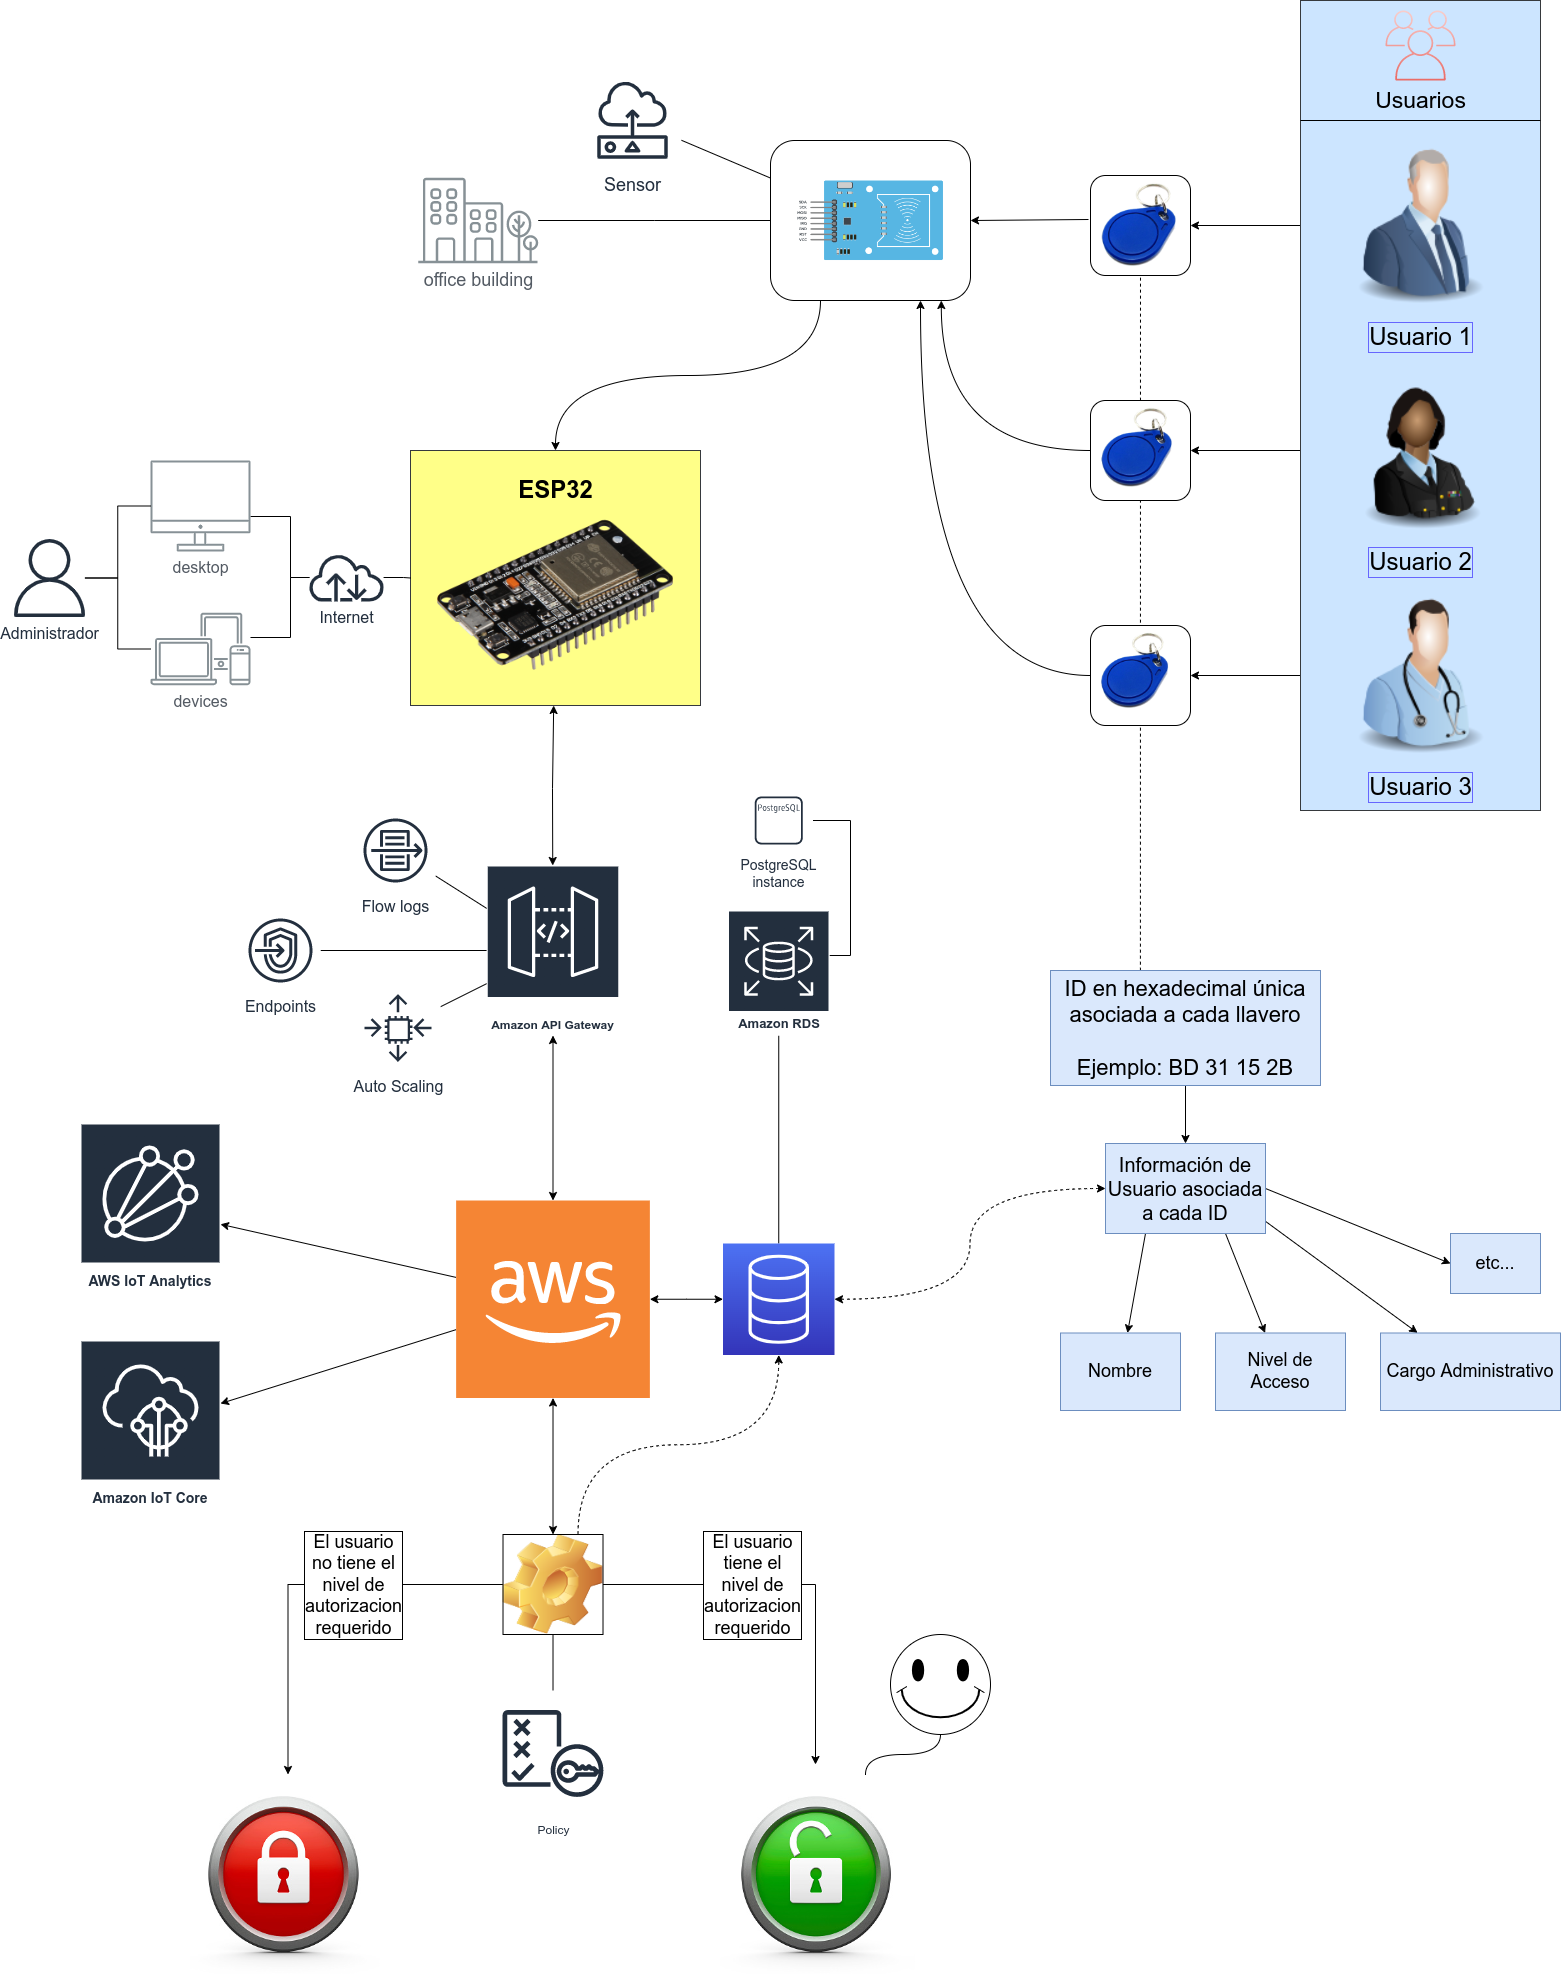
\includegraphics[width=0.85\textwidth]{diagrama.drawio.png}
	\centering
	\caption{Un diagrama del modelo}
\end{figure}
\end{document}